\section{Gaussian Mixture Models}
In simple words, Gaussian Mixture Models combine gaussian models into a complex model by taking a mixture of $K$ multivariate Gaussian densities of the form:
$$
p(x)=\sum_{k=1}^K \pi_k N_m\left(x \mid \mu_k, \Sigma_k\right)
$$
where $\pi_k \geq 0, \sum_{k=1}^K \pi_k=1$, and $N_m\left(x |\mu_k, \Sigma_k\right)$ is the $m$-dim Gaussian density.\\
Each Gaussian component has its own mean vector $\mu_k$ and covariance matrix $\Sigma_k$.\\
The parameters $\pi_k$ are called the \textbf{mixing coefficients.}

\begin{figure}[H]
    \centering
    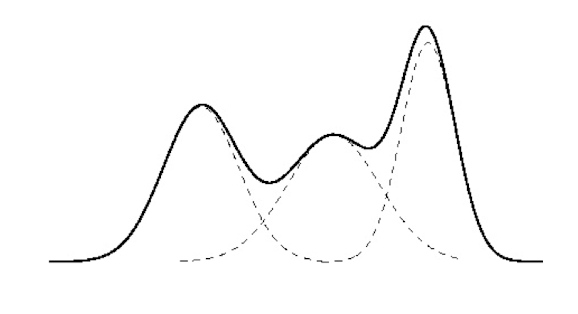
\includegraphics[width = .4\linewidth]{figures/section9/figure_9_1.png}
    \caption{An example of Gaussian Mixture Models}
    \label{fig:Gaussian-Mixture}
\end{figure}